\chapter{Case Study: L'approccio ibrido con tecnologie web}
\lhead{\emph{Capitolo 3}}
L'approccio ibrido con tecnologie web è stato scelto durante lo svolgimento del tirocinio presso la ditta BigThink SRL, in quanto si adattava meglio ad una serie di tecnologie già utilizzate dall'azienda per lo sviluppo di applicazioni multipiattaforma.
Durante la mia permanenza ho svolto il lavoro di Frontend Developer di Web Applications, in particolare mi occupavo dello sviluppo della logica di business di una applicazione e della sua interfaccia.
Una delle politiche dell'azienda era quella di separare la gestione dei dati e la loro memorizzazione lato Backend in modo tale che la parte Frontend sviluppata con il framework Javascript AngularJS si interfacciasse con i dati servendosi solo di API REST.
Dato il numero consistente di Web Application sviluppate e il mercato di applicazioni Mobile sempre in crescita, sono stato incaricato dall'azienda di ricercare dei metodi e delle tecnologie che consentissero di portare il lavoro già fatto per le Web Application su dispositivo mobile, in modo tale che l'azienda potesse offrire nuovi servizi.\\
Tutte le applicazioni sviluppate fino ad allora erano già Responsive Web Application, e ci si è posti l'obiettivo di aggiungere funzionalità caratteristiche dei dispositivi mobili, tramite l'utilizzo di tecnologie web.\\

Un primo punto di riferimento come tecnologia Web è stato AgnularJS, framework già utilizzato dall'azienda, se fosse stato scelto un altro framework si sarebbe dovuto riscrivere tutto il codice delle Web Application già sviluppate fino ad allora. A questo punto  si trattava di scegliere le corrette tecnologie per includere al meglio il lavoro già svolto, in particolare un wrapper che avrebbe consentito un buon sviluppo dell'applicazione partendo da tecnologie web, senza influire su eventuali spese aziendali. 

Per quanto riguarda gli strumenti di sviluppo utilizzati la scelta rimane allo sviluppatore, nel mio caso ho preferito elencarne alcuni secondo me importanti utilizzati all'interno dell'azienda e scoperti durante l'attività di ricerca.

\section{Le Tecnologie Web utilizzate}
Il riferimento per la scelta di tecnologie web è stato il framework \emph{AngularJS}, il quale è utilizzato a sua volta all'interno di altri framework, come ad esempio \emph{Ionic} che fornisce degli strumenti per la creazione di interfacce utente. Come wrapper ho scelto \emph{Cordova}, in quanto oltre ad essere un progetto open-source fornisce delle API per le funzionalità del dispositivo in linguaggio Javascript. Infine ho sperimentato una libreria chiamata \emph{ng-cordova}, la quale fornisce API per comunicare con il dispositivo ma con il codice già predisposto per AngularJS. 

\subsection{CSS Preprocessor}

Nei web framework che forniscono strumenti per la definizione di interfacce utente un componente che si trova molto spesso e il \emph{CSS Preporcessor} ovvero un preprocessore di fogli di stile.

\emph{In informatica, un preprocessore o precompilatore è un programma (o una porzione di programma) che effettua sostituzioni testuali sul codice sorgente di un programma, ovvero la precompilazione. I più comuni tipi di sostituzioni sono l'espansione di macro, l'inclusione di altri file, e la compilazione condizionale (vedi conditional compilation in inglese). Tipicamente, il preprocessore viene lanciato nel processo di compilazione di un software, e il file risultante verrà preso in input da un compilatore.}
\hspace*{\fill}\cite{wiki:preprocessor} 

\begin{figure}[htbp]
  \centering
    
\includegraphics[scale=0.25]{Figures/sass-logo.png} 
    
\includegraphics[scale=0.75]{Figures/less-logo.png} 
    \rule{35em}{0.5pt}
  \caption[Css Preprocessors]{\textbf{S}intatically \textbf{A}wesome \textbf{S}tyle\textbf{S}heet e \textbf{LESS}}
  \label{fig:CSS Preprocessors}
\end{figure}


Essendo CSS un linguaggio fortemente dichiarativo basato sui markup HTML, fa si che i fogli di stile per interfacce utente diventino molto lunghi e verbosi data la complessità delle interfacce utente. E di conseguenza risulta complesso applicare la propria personalizzazione.
I CSS preprocessor mettono a disposizione un set di operazioni chiamate MACRO che durante la compilazione verranno sostituite con il linguaggio CSS prorpio. Queste MACRO consentono ad esempio di fare utilizzo di variabili, funzioni, tag parametrici, ereditarietà dei tag, pattern matching, namespaces.

Queste sono solo alcune delle opzioni messe a disposizione dei CSS preprocessors dipende dalle sviluppatore scegliere quello secondo lui più adatto in quanto sul mercato ne esistono diversi, i più famosi e utilizzati sono \textbf{SASS}(\textbf{S}intatically \textbf{A}wesome \textbf{S}tyle\textbf{S}heet) e \textbf{LESS}(write \textbf{LESS} do more) \ref{fig:CSS Preprocessors}.

\subsection{AngularJS}
\label{sec:angularjs}

\begin{wrapfigure}{r}{0.40\textwidth}
  \vspace{-65pt}
  \begin{center}
    
\includegraphics[scale=0.40]{Figures/angular-logo.png}
  \end{center}
  \vspace{-10pt}
  \caption{\\AngularJS framework logo}
  \label{fig:AngularJS}
  \vspace{10pt}
\end{wrapfigure}

\paragraph*{Definizione}
AngularJS è un framework Javascript che segue il pattern MVC(\ref{subsec:mvc}) ideato da \emph{Minsko Hevery}(Google) che estende il linguaggio HTML in un formato più espressivo e leggibile. È caratterizzato da un approccio dichiarativo alla programmazione ed è stato pensato per separare la logica di business di una applicazione dalla sua presentazione dei dati, infatti sono presenti tag HTML espliciti come \emph{ng-view} e \emph{ng-model} che consentono di sincronizzare i dati del modello con la vista indipendentemente dalla loro logica. AngularJS è stato pensato esplicitamente per lo sviluppo di web application è presenta una forte modularità dei suoi componenti, in modo da renderli indipendenti e testabili, rispetta infatti i principi \emph{SOLID} \citep{wiki:solid} della programmazione orientata agli oggetti.
Ecco le caratteristiche principali di questo framework:

\begin{description}

\item[Directives] AngularJS si basa su un sistema di direttive, ovvero dei nuovi tag HTML che estendono il linguaggio di markup. Come viene mostrato nell'esempio \ref{lst:directives-example} ci sono delle direttive già predisposte dal framework per inserire i componenti principali a disposizione.

\begin{code}[language=html,caption={Un esempio delle direttive standard di AngularJS},
				   label={lst:directives-example}]
 <html ng-app="myApp">
     <div ng-controller = "InfoController">
       <input name = "inputFirstName" ng-model = "user.firstName">
       <input name = "inputSecondName" ng-model = "user.secondName">
       <div class = "showInfo">
	     Hello my name is {{user.firstName}} {{user.secondName}}			
       </div>
     </div>
 </html>
\end{code}

AngularJS inoltre offre la possibilità di definire direttive personalizzate \ref{fig:custom-directive}. La differenza sostanziale rispetto ai semplici tag HTML è che ad ogni direttiva è associato un particolare comportamento dell'applicazione. Mentre nei tag HTML si specifica come un certo elemento debba apparire nella pagina, ad esempio se contiene una porzione di testo oppure un'immagine, con le direttive di AngularJS associamo un comportamento al tag ed eventualmente un template su cui basarsi.
Principalmente all'interno di una applicazione AngularJS le direttive vengono utilizzate per esprimere interfacce utente complesse, gestire eventi scatenati dall'interazione con l'utente, re-utilizzo dei componenti più comuni e la ridefinizione dei tag già in uso. La buona pratica del framework vuole che solo all'interno delle direttive si possa manipolare il DOM.

\begin{figure}[htbp]
  \centering
    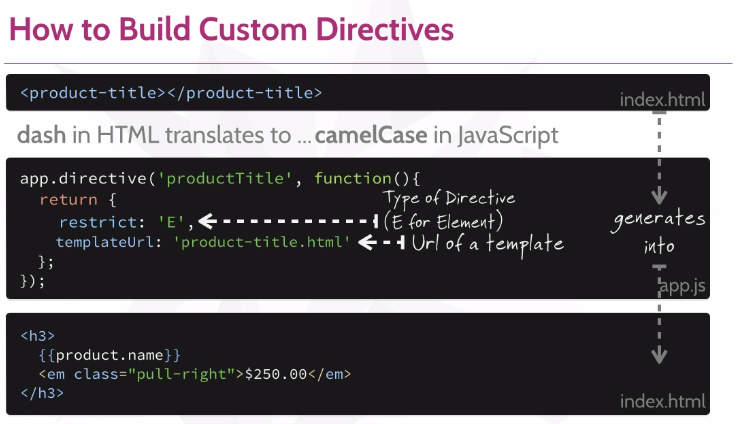
\includegraphics[scale=0.65]{Figures/how-to-build-custom-directives.png} 
    \rule{35em}{0.5pt}
  \caption[Custom Directive]{Creazione di una direttiva personalizzata}
  \label{fig:custom-directive}
\end{figure}

Una nota di sintassi particolare per le direttive riguarda il loro nome, come osserviamo il nome delle direttive nell'esempio \ref{fig:custom-directive} è separato dal trattino alto(\emph{dash}) mentre nella definizione tramite codice AngularJS è scritta in \emph{camelCase}. Questa è un convenzione che il framework adotta per evitare errori di sintassi all'interno del codice da parte del parser. Le direttive hanno a disposizione molte opzioni per essere personalizzate, per un trattazione più approfondita e completa si rimanda la lettura del manuale \cite{angularjs:directives}.

\item[Data Binding] Il Data Binding in AngularJS è la sincronizzazione automatica dei dati tra modello e vista. In modo in cui AngularJS implementa il data bindign consente di trattare il modello come SSOT(\cite{wiki:SSOT}). La vista è la proiezione del modello in ogni momento, quando il modello cambia la vista riflette il cambiamento e viceversa. 
La maggior parte dei sistemi di templating sincronizzano i dati in una sola direzione: si fondono componenti del template e modello insieme in una vista. Quando si verifica la fusione, le modifiche al modello o sezioni correlate della vista vengono NON si riflettono automaticamente nella vista. Peggio ancora, le eventuali modifiche che l'utente fa nella vista non si riflettono nel modello. Ciò significa che lo sviluppatore deve scrivere del codice apposito che sincronizza costantemente la vista con il modello e il modello con la vista.

\begin{figure}[htbp]
  \centering
    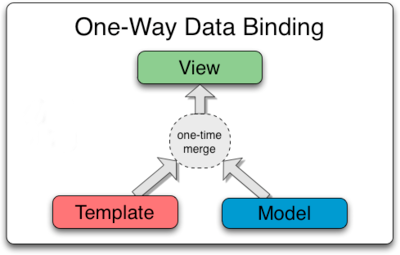
\includegraphics[scale=0.5]{Figures/one-way-data-binding.png} 
    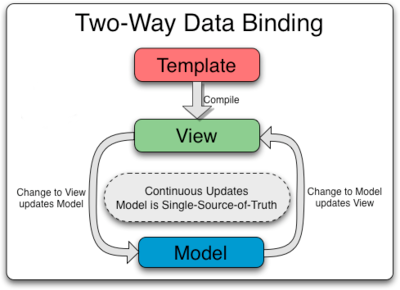
\includegraphics[scale=0.5]{Figures/two-way-data-binding.png} 
    \rule{35em}{0.5pt}
  \caption[Data Bindings]{Come è strutturato un classico data binding, e come invece è fatto in AngularJS}
  \label{fig:Data Binding}
\end{figure}

In particolare come si vede nell'esempio \ref{lst:directives-example} il binding dalla vista al modello è effettuato tramite la direttiva \emph{ng-model = "nome-del-modello"}, mentre dal modello alla vista si utilizza la sintassi \emph{ \{\{nome-del-modello\}\} }.

Il sistema dei template di AngularJS funziona in modo differente. In primo luogo il modello (che è l'HTML non compilato insieme a  markup o direttive supplementari) viene compilato sul browser. Il passo di compilazione produce una live view(vista). Eventuali modifiche alla vista si riflettono immediatamente nel modello, e le eventuali modifiche nel modello vengono propagate alla vista. Il modello è il SSOT per lo stato dell'applicazione, semplificando notevolmente il modello di programmazione per lo sviluppatore. Si può pensare di vista semplicemente come una proiezione istantanea del modello.

Poiché la vista è solo una proiezione del modello, il controller è completamente separato dal punto di vista e completamente allo scuro di essa. Questo rende i test dell'applicazione molto semplici, in quanto è facile testare il controller indipendentemente dalla vista e dalla relativa dipendenza dal DOM / browser web.

\item[Controller] i controller in AngularJS hanno il compito di gestire la logica di una determinata sezione dell'applicazione. Quando un controller viene dichiarato su una parte del DOM tramite la direttiva \emph{ng-controller} come nell'esempio \ref{lst:newController} AngularJS crea un nuovo oggetto Javascript associandogli un nuovo scope che potrà essere inserito all'interno del controller tramite la dependency injection. 

\begin{code}[caption={Associazione tra un elemento del DOM e un controller}, label={lst:newController}]
	<div id="header" ng-controller = "HeaderController"></div>
\end{code}

In generale ci sono alcune regole da seguire per la creazione dei controller, le quali non sono obbligatorie ma sono considerate come si dice in gergo \emph{Best Practices}:
I controller devono essere usati per:

\begin{itemize}
\item Configurare lo stato iniziale dello scope.
\item Aggiungere comportamento allo scope(funzioni, modelli, oggetti)
\end{itemize}
Mentre i controller non devono essere usati per:
\begin{itemize}
\item Manipolare elementi del DOM
\item Formattare input e output
\item Condividere codice tra i vari controller.
\item Gestire il ciclo di vita degli altri componenti(creazione di nuove istanze)
\end{itemize}

\item[View] In base ai contenuti e al template scelto per visualizzarli AngularJS genera una vista, che non è altro che la proiezione dei dati in un certo momento dell'applicazione. Inoltre grazie ad un meccanismo di routing, è possibile impostare un workflow dell'applicazione specificando le varie viste possibili, anche in maniera gerarchica. 

\item[Dependency Injection] per una trattazione generale dell'argomento rimandiamo all'appendice \ref{app:DepInj}. AngularJS ha già al suo interno un meccanismo che gestisce la Dependency Injection. Il principale scopo per cui AngularJS è stato dotato di questa caratteristica è per avere la possibilità di suddividere in moduli separati l'applicazione dove ognuno di essi può essere iniettato all'interno degli altri e vice versa. Un esempio moto semplice di Dependency Injection in AngularJS è all'atto della creazione dell'applicazione. Nell'esempio \ref{lst:appCreation} il metodo \textit{angular.module()} prende due argomenti: il primo è il nome del modulo che si vuole creare, mentre il secondo è un array con tutti i moduli di cui è composto la nostra applicazione. Viene creato quindi un riferimento ai moduli inclusi e non un istanza diretta.  

\begin{code}[caption = {Creazione di una applicazione in AngularJS con le relative dipendenze}, 
				   label = {lst:appCreation}]
	var testApp = angular.module("testApp",['ngRoute','customModule']);
\end{code}

Oltre ai moduli AngularJS da la possibilità di usare la propietà della Dependency Injection sui tipi base forniti dal linguaggio, ovvero:

\begin{itemize}
\item Value
\item Factory
\item Service
\item Provider
\item Constant
\end{itemize}

Un esempio di Dependency Injection di questi tipi avviene molto frequentemente nelle applicazioni all'interno dei controller (\ref{lst:controllerExample})

\begin{code}[caption = {Un esempio di creazione di un modulo e la sua inclusione all'interno di un altro}, 
				   label = {lst:controllerExample}]

angular.module("CustomModule",[])
.service("CustomService",function(){
	this.customMethod = function(value){
		return value + " from customMethod in CustomService";	
	}
});

angular.module("testApp",[
	'CustomModule'
]).controller("HomeController", function(CustomService){
	CustomService.customMethod("Marco");
});

\end{code}

\item[Service] si è visto come il meccanismo di Dependency Injection possa rendere disponibile all'interno dell'applicazione tutti i componenti forniti da un specifico modulo. Fatta eccezione per i \emph{service} ogni volta che si richiama un componente tramite Dependency Injection dal riferimento viene creata una nuova istanza della classe. I service invece sfruttano quello che è chiamato in Javascript il \emph{Singleton Object}, ovvero, l'istanza di un oggetto di tipo service avviene soltanto una volta, e il riferimento all'interno dell'applicazione è univoco verso lo stesso oggetto(figura \ref{fig:AngularJS-Singleton}). Inoltre soltanto quando il service dipende dall'applicazione viene creata l'istanza dell'oggetto(\emph{Lazy Initialization}).

\begin{figure}[htbp]
  \centering
    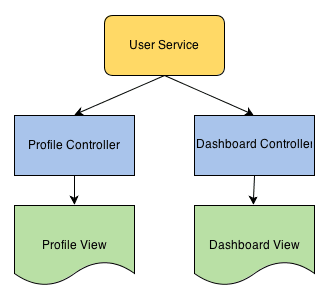
\includegraphics[scale=0.75]{Figures/angularjs-service-singleton-diagram.png}  
    \rule{35em}{0.5pt}
  \caption[AngularJS Singleton]{Schema di come è strutturato un service all'interno di AngularJS}
  \label{fig:AngularJS-Singleton}
\end{figure}

I service possono essere creati dallo sviluppatore oppure AngularJS ne mette a disposizione già alcuni, come ad esempio \emph{\$http} che è uno dei più usati per lo scambio dei dati attraverso l'omonimo protocollo. Altro uso dei service può essere quello dello scambio dei dati attraverso i controller, genericamente in una applicazione che si interfaccia con dei servizi backend e buona norma associare ad ogni servizio corrispettivo un service di AngularJS.

\item[Provider/Factory/Service] una trattazione separata di queste tre caratteristiche di AngularJS potrebbe risultare difficile da comprendere. Avendo spiegato cosa è un service la trattazione prosegue su altri due componenti strettamente correlati: i Factory e i Provider.
Tra questi tre componenti esiste una specie di gerarchia : i \textit{service} sono degli oggetti singleton creati tramite una \textit{factory}. Le \textit{factory} sono funzioni che a sua volta sono create tramite un \textit{provider}. I \textit{provider} sono dei costruttori che hanno a disposizione un metodo \emph{\$get} il quale contiene la \emph{service factory} che ritorna l'istanza del service.

In questo modo AngularJS si garantisce una forte modularizzazione dei componenti, e la ricerca dei corretti riferimenti da parte della Dependency Injection. Inoltre tramite il provider è possibile configurare, se previsto, i servizi dell'applicazione scrivendo un opportuno codice parametrico.

\end{description} 


\subsection{Ionic}

\begin{wrapfigure}{r}{0.40\textwidth}
  \vspace{-65pt}
  \begin{center}
    
\includegraphics[scale=0.35]{Figures/ionic-logo.png}
  \end{center}
  \vspace{-10pt}
  \caption{Ionic Framework Logo}
  \label{fig:IONIC}
  \vspace{-10pt}
\end{wrapfigure}
IONIC è un UI Framework basato sulle tecnologie web HTML5, Sass, AngularJS per la creazione di interfacce utente per dispositivi mobili. Si basa sul sistema di direttive di AnagularJS è fornisce un nuovo set di tag HTML componibili tra di loro. 
Gli UI Framework e IONIC principalmente dispongono di 3 categorie di elementi che li caratterizzano e che servono per l'appunto alla composizione dell'interfaccia utente:

\begin{description}

\item[CSS Components] Sono dei componenti statici creati tramite HTML e CSS come bottoni, barre di navigazione, liste, tabelle che possono essere assemblati tra di loro come i componenti di una pagina web. I CSS di IONIC mettono a disposizione classi che possono cambiarne forma, dimensione e colore che a loro volta possono essere combinate.
Per personalizzazioni più avanzate e possibile seguire una guida messa a disposizione dal framework che spiega come modificare i file di Sass e che caratteristiche si va a cambiare(come ad esempio i colori standard).

\item[Javascript Components] Al fine di offrire una esperienza di una applicazione mobile all'utente, IONIC offre delle estensioni in AngularJS che ricalcano quelle che sono le operazioni e le interfacce più comuni sui i dispositivi mobili. Ispirato ai sistemi iOS e Android questo framework mette a disposizione componenti come gestori di eventi, paginazione dei contenuti, popup di sistema, touch gestures, menu laterali, scorrimento di pagine il tutto nello stile di una applicazione mobile vera e prorpia.

\item[Ionicons] IONIC prevede un set di icone standard che possono essere utilizzate all'interno dei componenti e personalizzate a proprio piacimento.

\end{description} 

\section{Il Wrapper Framework}
Come spiegato nella sezione \ref{sec:appAndFramework} per lo sviluppo di applicazioni multipiattaforma si necessita di un framework che possa in qualche modo tradurre il linguaggio originale in quello della specifica piattaforma.
Nel caso di una applicazione ibrida, si ha bisogno di un framework che possa ospitare tecnologie web e che abbia un interfaccia verso le funzionalità del dispositivo. Si ribadisce che non tutti i framework possono essere usati su tutte le piattaforme, bisogna scegliere con accortezza di quale servirsi.
Data la mia formazione come sviluppatore web presso l'azienda BigThink SRL ho scelto di utilizzare il framework \emph{Cordova} per i seguenti motivi:
\begin{itemize}
\item E' un framework che si adatta a sviluppatori web che vogliono portare le proprie applicazioni su dispositivi mobili, in quanto fornisce le varie API per le funzionalità del dispositivo in linguaggio Javascript.
\item E' open-source quindi costi di licenza nulli per l'azienda e per lo sviluppatore ed inoltre e seguito da una community popolata e attiva.
\item Supporta 16 piattaforme diverse con oltre 20 plugin per interagire con il dispositivo, assieme ad altre librerie per la creazione di plugin personalizzati.
\item Si integra al meglio con AngularJS grazie ad una libreria chiamata \emph{ng-cordova}(\ref{sec:ngCordova}).
\end{itemize}

\subsection{Cordova/Phonegap}

\begin{wrapfigure}{r}{0.40\textwidth}
  \vspace{-65pt}
  \begin{center}
    
\includegraphics[scale=0.35]{Figures/cordova-logo.png}
  \end{center}
  \vspace{-10pt}
  \caption{\\Cordova Framework Logo}
  \label{fig:Cordova}
  \vspace{-30pt}
\end{wrapfigure}


Per chi magari è nuovo nel settore delle applicazioni multi-piattaforma, o per chi ci è entrato da poco 	avrà fatto sicuramente confusione tra queste due nomenclature \texttt{Cordova} e \texttt{Phonegap}, ecco quindi una delucidazione sul fatto.

\subsubsection{Storia}
Phonegap è stato creato nel 2009 da una startup chiamata \emph{Nitobi} come progetto open-source. Si proponeva di fornire un metodo per l'accesso alle funzionalità native del dispositivo tramite il meccanismo di wrapping che è stato discusso nel capitolo precedente a proposito dei framework. L'obiettivo di questa piattaforma era appunto quello di poter creare delle applicazioni che potessero essere usate nei dispositivi mobili, tramite l'utilizzo di tecnologie web come HTML5, CSS e Javascript, ma con ancora la possibilità di accedere alle funzionalità native del dispositivo.\\
Nel 2011 \emph{Adobe} ha acquisito la startup Nitobi assieme ai diritti di Phonegap, e il codice open-source della piattaforma è stato donato all'\emph{Apache Software Foundation} con il nome di \texttt{Cordova}

\begin{figure}[!ht]
  \centering
    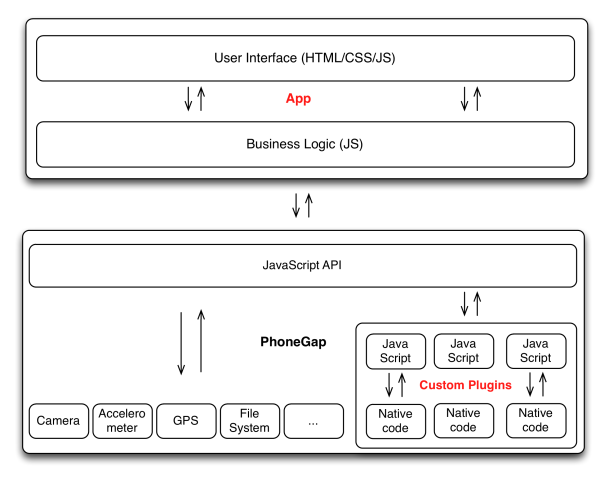
\includegraphics[scale=0.65]{Figures/cordova_schema.png} 
    \rule{35em}{0.5pt}
  \caption[Struttura a Livelli di Cordova]{Come avviene le stratificazione tra l'applicazione e il framework Cordova}
  \label{fig:cordova-layers}
\end{figure}

\subsubsection{Differenze}
La vera differenza tra \texttt{Cordova} e \texttt{Phonegap}, viene descritta da \emph{Adobe} analogamente come la differenza tra \texttt{Blink}\footnote{Blink è la web browser engine di Google Chrome\cite{wiki:blink}} e \emph{Google Chrome}. Ovvero \emph{Cordova} e il cuore della piattaforma mentre \emph{Phonegap} aggiunge a \emph{Cordova} delle funzionalità proprietarie di \emph{Adobe}.\\
Personalmente ho scelto di utilizzare \emph{Cordova} per essere libero da qualsiasi vincolo proprietario.

\subsubsection{Cordova Core}
Cordova quindi offre una serie di potenti API in linguaggio Javascript per poter accedere alle funzionalità native del dispositivo. In difesa dello sviluppo nativo alcuni programmatori accusano \emph{Cordova} di non possedere tutte le possibilità di accesso a basso livello che invece si avrebbero. \emph{Cordova} è una realtà open-source e in quanto tale si è evoluta nel tempo offrendo sempre più funzionalità che hanno chiuso i divario che si credeva esservi tra questi due tipi di approcci.

Nella figura \ref{fig:cordova-layers} si può osservare dove si posiziona il framewrok all'interno di una tipica struttura stratificata di applicazione, e di come i livelli siano completamente indipendenti l'uno dall'altro. Questo fa si che per l'approccio cross-platform attraverso le applicazioni ibride, la scelta delle tecnologie web sia completamente irrilevante ai fini della creazione dell'app.

\subsection{ngCordova}
\label{sec:ngCordova}
\begin{wrapfigure}{r}{0.40\textwidth}
  \vspace{-65pt}
  \begin{center}
    
\includegraphics[scale=0.35]{Figures/ngcordova-logo.png}
  \end{center}
  \vspace{-10pt}
  \caption{\\ngCordova Logo}
  \label{fig:ngCordova}
  \vspace{0pt}
\end{wrapfigure}

Il perché in questa tesi si parli di \emph{Cordova} e \emph{AngularJS} è dato dall'esistenza di \texttt{ngCordova}. Questa libreria nasce da una idea di Paolo Bernasconi e Max Lynch che hanno avuto l'idea di unire la l'efficenza e la potenza di \emph{AngularJS} con la versatilità di \emph{Cordova}. Ne è nato un framework per lo sviluppo di applicazioni ibride direttamente collegato alle funzionalità del dispositivo gestibile tramite il codice efficiente di \emph{AngularJS}.\\

\begin{figure}[ht]
  \centering
    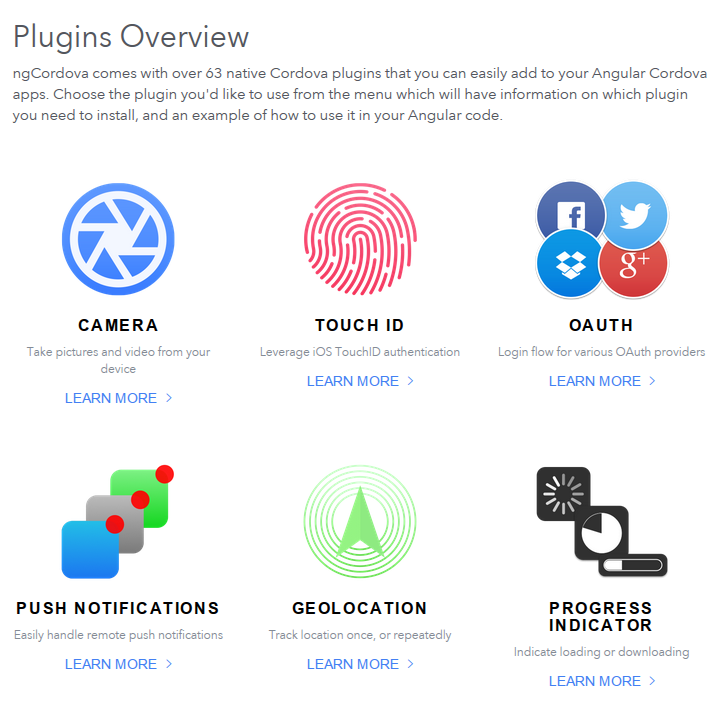
\includegraphics[scale=0.66]{Figures/ngcordova-plugins.png} 
    \rule{35em}{0.5pt}
  \caption[ngCordova Plugin]{Le principali categorie dei plugin di ng-corodva}
  \label{fig:ngcordova-plugins}
\end{figure}

Nell'architettura mostrata nella figura \ref{fig:cordova-layers} ng-cordova si posiziona al di sopra delle API di Cordova, ridefinendo i plugin nella sintassi di AngularJS. 

\section{Strumenti di sviluppo}

Il consistente numero di tecnologie che si possono utilizzare per lo sviluppo ibrido viene spesso accompagnato da strumenti che consentono di creare un ambiente progettuale in cui si ha a disposizione tutto il necessario per poter iniziare a sviluppare. La scelta di determinati strumenti piuttosto che altri è riservata allo sviluppatore finale, personalmente mostrerò come ho deciso di organizzare un progetto di esempio.

\subsection{Package Manager}

Avendo a disposizione tutto il mondo delle tecnologie web, può risultare utile e molto produttivo inserire librerie all'interno del nostro progetto. Per le applicazioni web in generale e anche in quelle ibride si può disporre di un package manager che facilmente includere nuove librerie all'interno del progetto.\\

\textbf{Bower} è un package manager tipicamente usato per librerie Javascript. Generalmente è possibile reperire ogni libreria disponibile su Github. Tramite il file \emph{bower.json} possiamo specificare le dipendenze del progetto e dinamicamente aggiornare la lista delle librerie installate. Inoltre se stiamo lavorando con una struttura di cartelle specifica, come ne mio caso, possiamo specificare la posizione di dove verranno scaricate le librerie tramite il file \emph{.bowerrc}. 

\begin{code}[language=html,caption={Una tipica configurazione del file .bowerrc},
				   label={lst:bowerrc}]
	{
		"directory" : "js/vendor"
	}
\end{code}

\begin{code}[language=html,caption={Una tipica configurazione del file bower.json},
				   label={lst:bowerjson}]
{
  "name": "blog.marcopredari.it",
  "version": "0.0.0",
  "authors": [
    "predorock <predorock@gmail.com>"
  ],
  "description": "A simple blog with angularJS",
  "main": "index.html",
  "license": "MIT",
  "homepage": "blog.marcopredari.it",
  "private": true,
  "ignore": [
    "**/.*",
    "node_modules",
    "bower_components",
    "test",
    "tests"
  ],
  "dependencies": {
    "angular-sanitize": "~1.3.10",
    "angular": "~1.3.10"
  }\begin{minipage}[\linewidth]
}

\end{code}


\subsection{Task Runner}
\label{sec:task_runner}
\begin{wrapfigure}{r}{0.40\textwidth}
  \vspace{-65pt}
  \begin{center}
    
\includegraphics[scale=0.4]{Figures/grunt-logo.png}
	
\includegraphics[scale=0.3]{Figures/gulp-logo.png}  
  \end{center}
  \vspace{-10pt}
  \caption{Loghi di Grunt e Gulp}
  \label{fig:task runner}
  \vspace{0pt}
\end{wrapfigure}

La divisione logica in moduli di una applicazione porta i programmatori a separare in file diversi l'applicazione in fase di sviluppo. Per poter ottenere una versione in fase di produzione occorre assemblare tutte le parti del progetto e se necessario eseguire dei test.
Il ruolo dei task-runner è quello di eseguire determinate operazioni per la messa in produzione dell'applicazione, come la concatenazione dei file, controllo della sintassi, test sui moduli e lo spostamento del progetto nella directory finale.

\textbf{Grunt} e \textbf{Gulp} sono due esempi di \emph{task-runner} in linguaggio Javascript(NodeJs). Una caratteristica che li distingue e la loro modularità, in quanto in base alle esigenze dell'applicazione si possono scaricare i moduli dedicati in base ai processi richiesti per la messa in produzione. Successivamente si deve scrivere un file(\textit{grunt.js} o \textit{gulp.js}) dove si indicano tutte le istruzioni per la messa in produzione. Ho voluto nominarli entrambi nella mia tesi in quanto il primo l'ho usato durante la mia esperienza di tirocinio, il secondo invece è usato per lo sviluppo del framework Ionic.


\section{SDK}
Un \texttt{Software Developement Kit} in generale è un insieme di strumenti per lo sviluppo e la documentazione del software\cite{wiki:sdk}. Questi strumenti vengono rilasciati dalla casa produttrice di una certa piattaforma come librerie di riferimento per lo sviluppo di software specifico di essa. La loro distribuzione avviene in uno specifico linguaggio a seconda della piattaforma ed è sempre affiancata da una documentazione molto accurata. 
Per lo sviluppo di applicazioni ibride avremo bisogno di ciascuna \emph{SDK} per ogni sistema operativo sul quale vorremo la nostra applicazione; ad esempio se volessimo la nostra applicazione per \emph{iOS} e \emph{Android} dovremmo scaricare entrambe le \emph{SDK}(scritte rispettivamente in C++/Swift e Java) indicando dove si trovano all'interno del notro computer.

\section{Pattern Javascript e best practices}
Per lo sviluppo di applicazioni ibride come si è notato il linguaggio che gestisce la logica dell'applicazione è senza dubbio Javascript. In risposta ai problemi che ho riscontrato durante la fase di sperimentazione ho raccolto una serie di pattern / best-practices secondo me utili allo sviluppo ibrido.
 
\subsection{Utilizzo delle Promises}
Una promise rappresenta un'interfaccia di delegazione verso un valore non ancora conosciuto. Essa consente di associare due tipi di comportamento ad una azione asincrona, nel caso di successo oppure di fallimento. \citep{mdn:promise}
Questo pattern e molto usato nel caso di chiamate ad API REST, molto spesso le risorse si trovano su un altro dominio che impiega un certo tempo a fornire il risultato. Mentre nello sviluppo ibrido vengono utilizzate per la chiamata alle API dei vari plugin associati ad una funzionalità del dispositivo.

\begin{code}[label={lst:promise_ex}, caption={Un esempio di uso delle promises in ng-cordva}]
 module.controller("PictureCtrl",function($scope, $cordovaCamera){
   document.addEventListener("deviceReady",function(){
     var options = {
       quality: 50,
       destinationType: Camera.DestinationType.DATA_URL,
       sourceType: Camera.PictureSourceType.Camera
       allowEdit: true,
       encodingType: Camera.EncodingType.JPEG,
       targetWidth: 100,
       targetHeight: 100,
       popoverOptions: CameraPopoverOptions,
       saveToPhotoAlbum: false
     };
   $cordovaCamera.getPicture(options).then(
      function(imageData){
       var image = document.getElementById('myImage');
       image.src = "data:image/jpeg:base64" + imageData;
      },
      function(err){
       alert("Something has gone wrong because :" + err);
      }
     ;
    }, false);
   });
$
\end{code}

Come si può vedere nell'esempio \ref{lst:promise_ex} la funzione \emph{.then()} viene applicata ad una promise che gestisce i dati provenienti dalla fotocamera di un dispositivo. Successivamente vengono specificate le due funzioni nel caso di successo o nel caso di errore della chiamata all'API.

\subsection{Stato dell'applicazione}
In una applicazione ibrida basata su Cordova esistono degli stati nei quali l'applicazione si può trovare. Come mostra la figura \ref{fig:cordova_app_states} durante la transizione degli stati vengono scatenati degli eventi che possono essere gestiti tramite codice Javascript.

\begin{figure}[htbp]
  \centering
    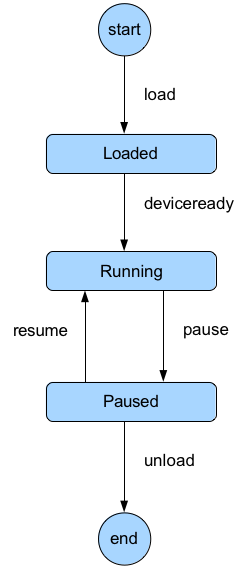
\includegraphics[scale=0.6]{Figures/cordova_application_states.png}  
    \rule{35em}{0.5pt}
  \caption[Stati di una applicazione]{Schema della transizione degli stati e degli eventi scatenati}
  \label{fig:cordova_app_states}
\end{figure}

L'evento più importante tra tutti è \emph{deviceReady} il quale indica che Cordova è stato caricato completamente e soltanto dopo questo evento possono essere richiamate le API per interagire con le funzioni del dispositivo. Gli eventi \emph{pause} e \emph{resume} indicano rispettivamente quando una applicazione viene messa in background e quando invece viene ripresa la sua esecuzione. Durante questi due eventi si può ottimizzare la gestione della memoria da parte dell'applicazione per non appesantire di calcoli il dispositivo. Ulteriori eventi che possono essere scatenati dalla pressione di pulsanti oppure da informazioni riguardo lo stato della batteria o quello della rete sono disponibili sulla documentazione \citep{web:phonegap_events}.

\subsection{Routing}
Un buona pratica in una applicazione ibrida, quando si utilizzano tecnologie web, è definire la struttura di navigazione tra le viste dell'applicazione. Tramite il \emph{\$routeProvider} messo a disposizione si possono configurare i cambiamenti di stato tra una vista e l'altra, assegnando per ciascuna di esse il template e il controller da caricare. Esiste anche un meccanismo più avanzato utilizzato da IONIC specifico per le applicazioni mobile chiamato \emph{\$stateprovider} detto anche \emph{angular-ui-router}. Le differenze principali dal routing originale di AngularJS sono che uno \textit{stato} corrisponde ad un determinato posto all'interno dell'applicazione nei termini della User Interface e della navigazione. Uno \textit{stato} descrive, tramite il controller, il template e le proprietà della view, l'aspetto della UI e il suo comportamento in quel posto. Può esistere una struttura gerarchica degli stati per cui alcuni possono trovarsi all'interno di altri. \citep{angularjs:ui-router} 

\subsection{OAUTH}
OAUTH è un protocollo sviluppato alla fine del 2012 per lo scambio di dati sensibili attraverso servizi di terze parti \citep{rfc:oauth}. In ambito web è conosciuto per il suo ampio uso nell'autenticazione attraverso provider differenti, ovvero grazie a questo protocollo e possibile autenticarsi ad un servizio / applicazione attraverso un altro di questi dove si è già registrati. Un esempio lampante è l'autenticazione tramite il proprio account di facebook, molto spesso le applicazioni per ovviare la pigrizia di alcuni utenti a registrarsi al loro servizio, mettono a disposizione un bottone tramite il quale l'utente acconsente che un provider, in questo caso facebook, possa fornire all'applicazione i dati necessari all'autenticazione o registrazione.
OAUTH garantisce uno scambio di dati protetto con la massima semplicità. È presente un plugin in ng-cordova per l'autenticazione verso i provider più comuni.
